\documentclass[11pt]{beamer}
\usetheme{Madrid}
\usepackage[utf8]{inputenc}
\usepackage{amsmath}
\usepackage{amsfonts}
\usepackage{amssymb}
\usepackage{graphicx}
\usepackage{algorithmic}
\usepackage{algorithm}
\usepackage{listings}

\DeclareMathOperator {\argmin}{argmin}

\author{Hongda Li}
\title{TSP via Dynamic Programming}
% Informe o seu email de contato no comando a seguir
% Por exemplo, alcebiades.col@ufes.br
\newcommand{\email}{email}
%\setbeamercovered{transparent}
\setbeamertemplate{navigation symbols}{}
%\logo{}
\institute[]{UBCO}
\date{\today}
%\subject{}

% ---------------------------------------------------------
% Selecione um estilo de referência
\bibliographystyle{plain}

%\bibliographystyle{abbrv}
%\setbeamertemplate{bibliography item}{\insertbiblabel}
% ---------------------------------------------------------

% ---------------------------------------------------------

\begin{document}

\begin{frame}
    \titlepage
\end{frame}

\begin{frame}{ToC}
    \tableofcontents
\end{frame}

\section{Introduction}
    \begin{frame}{Introduction}
        Define $G=(V, E)$ to be an undirected graph. 
        \begin{itemize}
            \item [1.] Dynamic programming is the idea of combining optimal solutions for smaller problems to make the full solution. 
            \item [2.] For the traveling salesman, we consider using spanning paths for covering different sizes of subsets. 
        \end{itemize}
        \begin{definition}
            Let $S\subseteq V$ and use $C(S, i, j)$ to denote the optimal $i\rightarrow j$ spaning path and its cost covering all vertices in $S$. 
        \end{definition}
    \end{frame}
    \begin{frame}{The algorithm}
        \begin{block}{TSP using Dynamic Programming}
            \begin{algorithm}[H]
                \caption{Held Karp algorithm for Travelling Salesman}\label{alg:dtsp}
                \begin{algorithmic}
                    \FOR{$i, j\in V, i < j$}
                    {
                        \STATE{C(\{i, j\}, i, j)} := c(i, j)
                    }
                    \ENDFOR
                    \FOR{$k = 3,4, \cdots n$}
                    {
                        \FOR{$|S| = k, S\subseteq V$}
                        {
                            \FOR{$i, j \in S, i < j$}
                            {
                                \STATE
                                {$C(S, i, j) := \min_{l\in S\setminus \{i, j\}} \{
                                    C(S\setminus \{j\}, i, l) + c(l, j)
                                \}$
                                }
                            }
                            \ENDFOR
                        }
                        \ENDFOR
                    }
                    \ENDFOR
                    \STATE{\textbf{return }$\min_{i, j \in V}
                        \{C(V, i, j) + c(i, j)\}$}
                \end{algorithmic}
            \end{algorithm}    
        \end{block}
    \end{frame}
    \begin{frame}{Facts about the algorithm}
        \begin{itemize}
            \item [1.] Its complexity is $\mathcal{O}(n^32^n)$. 
            \item [2.] We need to keep track of the optimal solutions and the cost of the optimal solutions during the iterations of the algorithm. 
            \item [3.] Because this dynamic programming is a bottom-up approach, storing the results from previous iterations suffices. We used this strategy for our implementations. 
        \end{itemize}
    \end{frame}
\subsection{Implementations and some more details}
    \begin{frame}{Challenges and their solutions}
        \begin{itemize}
            \item [1.] Generating all subsets $S$ with size $k$ from $V$. 
            \item [2.] Choosing the data structure for $C(S, i, j)$. 
            \item [3.] Writing it out while the advisor pushes hard on the seminar presentations while being distracted by a cooler project for another class and the usual graduate school pain. 
            \item [4.] The perfectionist tendency. 
        \end{itemize}
        \pause
        \begin{block}{Solution}
            Solution: Use python and pythonic code. 
        \end{block}
    \end{frame}
    \begin{frame}{k-subsets}
        This is the inner function of another function that generates subsets given an array. It's a recursive yield function. 
        \begin{center}
            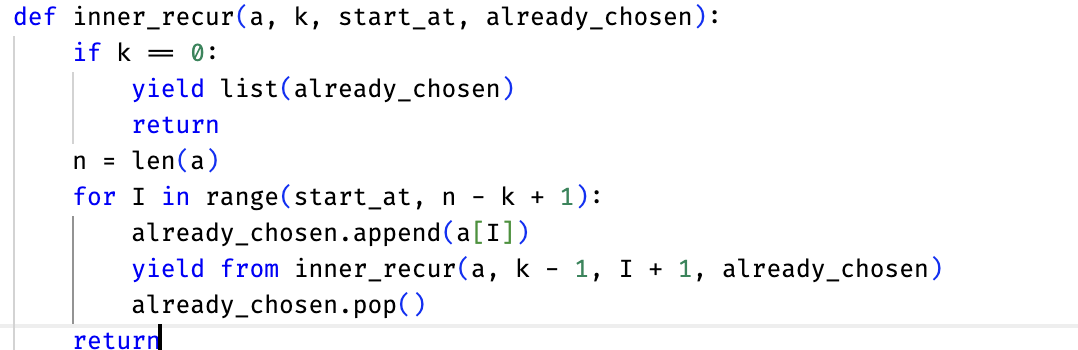
\includegraphics[width=12cm]{k_subsets.png}    
        \end{center}
    \end{frame}
    \begin{frame}{Python Itertools}
        When I first wrote this, I am unaware of the fact that python ``itertools'' exists and they provides generator for subsets and permutations. 
        \vspace{2em}
        \par
        Link is \href{https://docs.python.org/3.10/library/itertools.html}{\textcolor{blue}{here}}. Let's explore it together. 
    \end{frame}
    \begin{frame}{Storing the subsets and i, j}
        
    \end{frame}
    



\end{document}s